\documentclass[11pt,letterpaper]{article}

\usepackage[utf8]{inputenc}
\usepackage[T1]{fontenc}
\usepackage[spanish,es-noshorthands]{babel}
\usepackage{mathptmx}
\usepackage{amsmath,amssymb}
\usepackage{graphicx}
\usepackage{booktabs}
\usepackage{longtable}
\usepackage{tabularx}
\usepackage{array}
\usepackage{geometry}
\usepackage{float}
\usepackage{caption}
\usepackage{enumitem}
\usepackage{xcolor}
\usepackage{setspace}
\usepackage{tikz}
\usetikzlibrary{arrows.meta,positioning}
\usepackage{algorithm}
\usepackage{algpseudocode}
\usepackage{microtype}
\usepackage[hidelinks]{hyperref}

\geometry{letterpaper,margin=2.5cm}
\onehalfspacing
\addto\captionsspanish{\renewcommand{\tablename}{Tabla}}
\addto\captionsspanish{\renewcommand{\figurename}{Figura}}
\captionsetup{font=small,labelfont=bf}
\setlist[itemize]{topsep=2pt,itemsep=2pt,parsep=0pt}
\setlist[enumerate]{topsep=2pt,itemsep=2pt,parsep=0pt}
\setlength{\parskip}{0.35em}

\title{Decodificación con modelos ocultos de Markov para el riesgo dinámico de incendio forestal: un estudio de simulación reproducible}

\author{
Oscar Alonso De la Pava Suarez\\
Anderson Jesus Ospina Cardona\\
Kevin Andrés Valencia Daza\\[0.5em]
\small Ingeniería de Software y Datos, IUDigital, Colombia\\
\small Curso de Simulación, Grupo de Trabajo 11\\
\small Docente asesor: Julián Andrés Loaiza López\\
\small \texttt{oscar.delapava@est.iudigital.edu.co}\\
\small \texttt{anderson.ospina@est.iudigital.edu.co}\\
\small \texttt{kevin.valencia@est.iudigital.edu.co}\\
\small Autor de correspondencia: Oscar Alonso De la Pava Suarez\\
\small Repositorio: \url{https://github.com/skards11/Simulacion/tree/main/AE2_HMM}
}

\date{12 de noviembre de 2026}

\begin{document}

\maketitle

\begin{abstract}
\noindent
El riesgo de incendio forestal suele representarse con indicadores estáticos de humedad, aunque su evolución temporal podría capturarse con un modelo oculto de Markov (HMM). Este trabajo evalúa, mediante simulación y con fines didácticos, si la estructura temporal de un HMM aporta una ventaja medible frente a un clasificador sin memoria. Se formaliza un HMM discreto de tres estados (Riesgo Bajo, Moderado y Extremo) y tres observaciones ordinales de humedad (Alta, Media y Baja), con \(A\), \(B\) y \(\pi\) fijos. Se comparan tres reglas pareadas sobre \(T=500\) pasos y \(N=2000\) secuencias: M0, Viterbi nominal; M1, baseline puntual sin memoria basado solo en \(B\); y M2, Viterbi sobre observaciones degradadas con \(B(m=0.5)\). Se reportan media, desviación estándar, mínimo, máximo, IC 95\,\%, Wilcoxon pareado, Holm--Bonferroni y delta de Cliff. M0 y M1 resultaron estadísticamente indistinguibles en macro-F1 (0.6602 frente a 0.6603; \(p=0.778\); \(\delta=-0.006\)), mientras que M2 cayó a 0.4989 (diferencia 0.1612; \(p<0.001\); \(\delta=1.0\)). La dominancia diagonal de \(B\) explica la equivalencia práctica entre Viterbi y la regla puntual; la degradación de las emisiones, en cambio, erosiona la decodificación. El aporte es un protocolo reproducible ---código, semillas, hashes y auditoría--- que muestra que la estructura de Markov no garantiza superioridad cuando las emisiones dominan. Los resultados son simulados y no constituyen predicción de incendios reales.

\vspace{0.4em}
\noindent\textbf{Palabras clave:} modelos ocultos de Markov; decodificación de Viterbi; riesgo de incendio forestal; simulación reproducible; sensibilidad de emisiones.
\end{abstract}

% ==================================================================
\section{Introducción}

\subsection{Contexto}

La humedad de la vegetación y del suelo es un indicador habitual del peligro de incendio forestal. En un escenario simplificado, esa humedad puede registrarse de forma ordinal ---Alta, Media o Baja--- y asociarse a estados latentes de riesgo ---Bajo, Moderado o Extremo--- que no se observan directamente. Un modelo oculto de Markov (HMM) permite representar esa relación mediante una cadena latente con persistencia temporal y un proceso de emisión que conecta cada estado con las observaciones disponibles \cite{rabiner1989}.

La representación del riesgo como proceso dinámico exige distinguir dos objetos: la secuencia de estados latentes \(S_{1:T}\), que evoluciona según una cadena de Markov, y la secuencia de observaciones \(O_{1:T}\), que pertenece al alfabeto de humedad \(V\). El HMM no demuestra que exista un riesgo físico medible; solo ofrece un mecanismo probabilístico para inferir etiquetas latentes a partir de evidencia ordinal. Esta distinción es central para evitar afirmaciones que el diseño no puede sostener.

\subsection{Planteamiento del problema}

El problema abordado es metodológico y computacional. Aun cuando un HMM parezca apropiado por incorporar memoria temporal, no existe garantía de que supere a una regla simple que clasifique cada observación con la probabilidad de emisión más alta. Si la matriz \(B\) es diagonalmente dominante, el argumento de máxima verosimilitud puntual puede coincidir con la ruta de Viterbi y la ventaja atribuida a la estructura de Markov quedaría confundida con el efecto de las emisiones. Además, si los parámetros se estiman y evalúan sobre los mismos datos, el efecto del aprendizaje se mezcla con el de la decodificación.

En este trabajo se aísla ese efecto mediante inferencia con \(A\), \(B\) y \(\pi\) fijos, secuencias sintéticas pareadas y un escenario de degradación controlada de \(B\). El objetivo no es predecir incendios reales, sino determinar en qué condiciones la estructura temporal aporta una diferencia medible y cómo cambia esa diferencia cuando las emisiones pierden separabilidad.

\subsection{Justificación}

La justificación es doble. Desde la formación en simulación, el ejercicio permite implementar y contrastar Forward, Forward--Backward y Viterbi, verificar supuestos y reportar incertidumbre con un protocolo auditable. Desde la metodología, evita una conclusión apresurada: que un modelo sea más complejo no implica que sea mejor. Comparar el HMM con un baseline sin memoria y con una versión degradada permite observar si la ganancia proviene de la dinámica latente o de la calidad de las emisiones.

\subsection{Objetivos}

\textbf{Objetivo general:} evaluar de forma reproducible la decodificación de un HMM discreto con parámetros fijos en un escenario didáctico de riesgo de incendio forestal, comparándola con un baseline sin memoria y con un escenario de emisiones degradadas.

\textbf{Objetivos específicos:}
\begin{enumerate}
  \item Formalizar el HMM \(\lambda=(S,V,A,B,\pi)\) y las distribuciones discretas que gobiernan la cadena latente y las observaciones.
  \item Implementar M0 (Viterbi nominal), M1 (baseline puntual sin memoria) y M2 (Viterbi sobre emisiones degradadas) en un diseño pareado con \(T=500\) y \(N=2000\).
  \item Reportar métricas descriptivas, pruebas pareadas y evidencia de reproducibilidad, y auditar cada cifra contra los artefactos de \texttt{outputs/}.
\end{enumerate}

\subsection{Aportes}

\begin{itemize}
  \item Un protocolo explícito con matrices, semillas, métricas y criterios de decisión verificables.
  \item Una comparación controlada que separa la estructura del modelo de la estimación de parámetros, porque los tres escenarios reciben parámetros fijos.
  \item Evidencia cuantitativa de que la dominancia diagonal de \(B\) puede volver indistinguibles a Viterbi y a una regla puntual sin memoria.
  \item Un paquete de reproducibilidad con código, pruebas, figuras a 300 dpi, hashes SHA-256 y una tabla de auditoría numérica.
\end{itemize}

\subsection{Preguntas de investigación}

\begin{enumerate}[label=\textbf{P\arabic*.}]
  \item ¿Cómo puede representarse el riesgo dinámico de incendio forestal a partir de niveles de humedad mediante un Modelo Oculto de Markov?
  \item ¿Cómo influyen los parámetros del modelo (\(A\), \(B\), \(\pi\)) y las distribuciones discretas en los resultados de decodificación?
  \item ¿Qué tan reproducible y sensible es el modelo frente a perturbaciones en la matriz de emisión (\(B\)) y frente a un clasificador baseline sin memoria?
\end{enumerate}

% ==================================================================
\section{Estado del arte}

\subsection{Alcance de la revisión}

La revisión se realizó sobre un corpus cerrado de ocho documentos recientes y dos referencias fundacionales. Los criterios de inclusión fueron: emplear un HMM o una variante declarada, describir el algoritmo de inferencia o estimación, reportar resultados cuantitativos y disponer del texto completo. No se consultaron bases bibliográficas externas; por tanto, el alcance es una revisión estructurada y reproducible, no una síntesis exhaustiva. Los metadatos que no aparecen en las fichas se marcan como \texttt{[NO VERIFICADO]}.

\subsection{Fundamentos}

Rabiner \cite{rabiner1989} sistematizó los tres problemas canónicos ---evaluación, decodificación y aprendizaje--- y presentó Forward--Backward, Viterbi y Baum--Welch como sus soluciones algorítmicas. Baum, Petrie, Soules y Weiss \cite{baum1970} establecieron la técnica de maximización que fundamenta la reestimación tipo EM conocida como Baum--Welch. Ambos trabajos son conceptuales y algorítmicos: ninguno reporta una comparación empírica entre decodificación con HMM y baselines simples en un problema ordinal.

\subsection{Aplicaciones y desarrollos recientes}

\textbf{Ambiente y agua.} Wanjala, Makokha y Khamala \cite{wanjala2025} aplicaron un HMM multivariado con emisiones gaussianas a propiedades ópticas de aerosoles y variables climáticas en Kenia (2000--2022), con estimación EM, selección por BIC y decodificación de Viterbi; el modelo de cinco estados (BIC \(=1380\)) identificó anomalías en el 5.08\,\% de los meses. Grammenos \cite{grammenos2025} modeló la ocurrencia diaria de lluvia en Ceará (Brasil) con HMM de emisiones Bernoulli y comparó especificaciones homogéneas y no homogéneas mediante AIC/BIC; el mejor ajuste incorporó una covariable climática en la observación (BIC \(=24700.55\)). Tran et al. \cite{tran2026} combinaron un HMM gaussiano de tres estados con una red LSTM de doble rama y atención para clasificar la calidad del agua costera en Vietnam, con 74.87\,\% de exactitud y 64.11\,\% de F1.

\textbf{Incertidumbre y robustez.} Nicosia \cite{nicosia2026} propuso los ``tubos tropicales de Viterbi'' para cuantificar la incertidumbre de trayectorias casi óptimas en tiempo \(O(TK^2)\); los validó en seis escenarios simulados y en trayectorias GPS/acústicas reales de murciélagos, con enriquecimientos de 2.25 y 0.27 para forrajeo y desplazamiento. Pouzo, Psaradakis y Sola \cite{pouzo2025} demostraron por vía asintótica y por simulación Monte Carlo que los parámetros de la ecuación observable se estiman consistentemente por cuasi-máxima verosimilitud incluso si se ignora la cadena de Markov, siempre que los regímenes sean estacionarios y las covariables estrictamente exógenas.

\textbf{Industria, salud y análisis secuencial.} Li, Qian y Wang \cite{li2013} acoplaron un HMM izquierda-derecha con mezclas gaussianas a una regresión FS-LSSVR para pronosticar la vida útil remanente en el benchmark C-MAPSS, con reconocimiento de condición entre 77.69\,\% y 100.00\,\%. Deb, Pandey y Pakray \cite{deb2026} propusieron un HMM cuántico para etiquetado gramatical y reportaron un F1 superior al HMM clásico, aunque la ficha consultada solo cubre las páginas iniciales hasta la Sección~2.2. Wang et al. \cite{wang2026} introdujeron StageGuard, una capa con decodificador de Viterbi semi-Markoviano y restricciones fisiológicas para la estadificación del sueño, que reduce la tasa de violación de transiciones de 3.6--12.3\,\% a 0.1--0.8\,\%.

\subsection{Síntesis comparativa}

La Tabla~\ref{tab:comparativa} resume los diez trabajos. Predominan los HMM continuos con emisiones gaussianas y el ciclo ``EM/Baum--Welch \(\rightarrow\) Viterbi''; los HMM discretos aparecen en aplicaciones con observaciones categóricas o binarias y solo un trabajo emplea un formalismo semi-Markoviano. Las métricas son heterogéneas (BIC/AIC, exactitud/F1, MAPE/BIAS, tasas de violación de transiciones) y casi nunca se reporta la distribución completa por réplica.

\begin{table}[H]
\centering
\caption{Síntesis comparativa de los diez trabajos revisados.}
\label{tab:comparativa}
\footnotesize
\setlength{\tabcolsep}{3pt}
\begin{tabular}{@{}p{0.6cm}p{2.8cm}p{2.7cm}p{3.3cm}p{2.4cm}p{3.0cm}@{}}
\toprule
Ref. & Dominio & Tipo de HMM & Inferencia / entrenamiento & Datos & Métricas clave\\
\midrule
\cite{rabiner1989} & Voz / ASR (revisión) & Discreto & Forward--Backward, Viterbi, Baum--Welch & No aplica & Sin métricas propias\\
\cite{baum1970} & Teoría estadística & Discreto & EM / Baum--Welch & Teoría & Convergencia teórica\\
\cite{wanjala2025} & Aerosoles y clima & Continuo gaussiano & EM, BIC, Viterbi & Reales 2000--2022 & BIC \(=1380\); 5.08\,\% anómalo\\
\cite{grammenos2025} & Lluvia (Ceará) & Discreto Bernoulli & EM, AIC/BIC, Viterbi & Reales + GCM & BIC \(=24700.55\)\\
\cite{nicosia2026} & Movimiento animal & Continuo (2 estados) & Viterbi + tubo tropical & Simulación + GPS/audio & Enriquecimiento 2.25 / 0.27\\
\cite{pouzo2025} & Econometría & Regímenes con covariables & QML asintótico y Monte Carlo & Simulados & Consistencia asintótica\\
\cite{tran2026} & Calidad de agua & Continuo + LSTM & Baum--Welch, Viterbi, atención & Reales (1{,}305) & Exactitud 74.87\,\%; F1 64.11\,\%\\
\cite{li2013} & RUL / PHM & Continuo LR-MG-HMM & Baum--Welch/EM, forward, FS-LSSVR & Reales C-MAPSS & Condición 77.69--100\,\%\\
\cite{deb2026} & POS tagging & Discreto cuántico & QHMM, mediciones parciales & Reales & F1 superior al clásico\\
\cite{wang2026} & Estadificación del sueño & Semi-Markoviano & Viterbi semi-Markoviano + DL & Reales (4 datasets) & TVR 0.1--0.8\,\%\\
\bottomrule
\end{tabular}
\end{table}

\subsection{Vacío identificado}

La literatura deja abierto un problema acotado: no hay evidencia controlada sobre si la estructura temporal de un HMM, con \(A\), \(B\) y \(\pi\) fijos, mejora la decodificación frente a reglas simples cuando las observaciones son ordinales y el número de estados es pequeño. Los estudios aplicados confunden el efecto del modelo con el de la estimación porque entrenan y evalúan sobre los mismos datos o sobre datos reales sin contraste pareado. Los estudios metodológicos abordan la incertidumbre \cite{nicosia2026}, la robustez asintótica \cite{pouzo2025} o la exposición algorítmica \cite{rabiner1989,baum1970}, pero no esa comparación. D5a cubre exactamente esa brecha: inferencia con parámetros fijos, secuencias pareadas y un baseline sin memoria.

% ==================================================================
\section{Marco teórico}

\subsection{Distribuciones discretas y verosimilitud}

Sea \(S_t\in S=\{s_1,\dots,s_K\}\) el estado latente en el paso \(t\) y \(O_t\in V=\{v_1,\dots,v_M\}\) la observación. El HMM discreto se especifica con:
\begin{align}
a_{ij} &= P(S_t=s_j\mid S_{t-1}=s_i), & \sum_{j=1}^{K}a_{ij}&=1,\\
b_i(k) &= P(O_t=v_k\mid S_t=s_i), & \sum_{k=1}^{M}b_i(k)&=1,\\
\pi_i &= P(S_1=s_i), & \sum_{i=1}^{K}\pi_i&=1.
\end{align}
La verosimilitud conjunta factoriza como
\begin{equation}
P(O_{1:T},S_{1:T}\mid\lambda)
=\pi_{s_1}\,b_{s_1}(o_1)\prod_{t=2}^{T}a_{s_{t-1}s_t}\,b_{s_t}(o_t),
\end{equation}
donde \(o_t\) es el índice de la observación en \(V\). Las distribuciones son discretas y categóricas; no se usan densidades ni umbrales físicos de humedad.

\subsection{Propiedad de Markov e independencia condicional}

La cadena latente satisface
\begin{equation}
P(S_t\mid S_{1:t-1})=P(S_t\mid S_{t-1}),
\end{equation}
y las observaciones satisfacen independencia condicional dado el estado:
\begin{equation}
P(O_{1:T}\mid S_{1:T},\lambda)=\prod_{t=1}^{T}P(O_t\mid S_t).
\end{equation}
Estos dos supuestos definen el modelo y explican por qué la decodificación puede explotar la persistencia sin modelar dependencias de orden superior.

\subsection{Tupla \(\lambda=(S,V,A,B,\pi)\)}

El modelo se denota \(\lambda=(S,V,A,B,\pi)\), donde \(S\) es el conjunto de estados, \(V\) el alfabeto de observaciones, \(A=[a_{ij}]\in\mathbb{R}^{K\times K}\), \(B=[b_i(k)]\in\mathbb{R}^{K\times M}\) y \(\pi=[\pi_i]\in\mathbb{R}^{K}\). Es importante subrayar que \(O_t\in V\): las observaciones pertenecen al alfabeto de humedad, no al conjunto de estados. Los estados son etiquetas latentes y no se miden directamente.

\subsection{Los tres problemas clásicos}

\textbf{Evaluación.} Calcular \(P(O_{1:T}\mid\lambda)\) con la recursión Forward:
\begin{equation}
\alpha_t(j)=b_j(o_t)\sum_{i=1}^{K}\alpha_{t-1}(i)a_{ij},
\qquad
P(O_{1:T}\mid\lambda)=\sum_{j=1}^{K}\alpha_T(j).
\end{equation}

\textbf{Decodificación.} Obtener la ruta más probable con Viterbi:
\begin{equation}
\delta_t(j)=\max_i\bigl[\delta_{t-1}(i)a_{ij}\bigr]b_j(o_t),
\qquad
\psi_t(j)=\arg\max_i\bigl[\delta_{t-1}(i)a_{ij}\bigr].
\end{equation}
La posterior marginal \(P(S_t=s_i\mid O_{1:T})\) se obtiene con Forward--Backward.

\textbf{Aprendizaje.} Estimar \(A\), \(B\) y \(\pi\) con Baum--Welch, la variante EM que maximiza la verosimilitud esperada.

\subsection{Alcance D5a}

El experimento aplica únicamente decodificación con parámetros conocidos (D5a). No se implementa Baum--Welch porque el objetivo es aislar el efecto de la estructura temporal y de las emisiones, no el de la estimación. Fijar \(A\), \(B\) y \(\pi\) elimina la variabilidad de inicialización, permite comparaciones pareadas exactas y hace que las diferencias observadas se atribuyan a la regla de decisión o al escenario de emisión.

% ==================================================================
\section{Metodología}

\subsection{Fases del protocolo}

La Tabla~\ref{tab:fases} describe las fases F1--F7, sus actividades y entregables verificables.

\begin{table}[H]
\centering
\caption{Fases metodológicas, actividades y entregables.}
\label{tab:fases}
\small
\begin{tabularx}{\textwidth}{@{}p{0.8cm}>{\raggedright\arraybackslash}X>{\raggedright\arraybackslash}p{5.8cm}@{}}
\toprule
Fase & Actividad & Entregable\\
\midrule
F1 & Definir alcance, preguntas P1--P3 y criterios de éxito & \texttt{decisiones.md}; Sección~1\\
F2 & Revisar el caso didáctico y las matrices de trabajo & \texttt{materiales/}; Sección~3\\
F3 & Formalizar el HMM y las distribuciones discretas & \texttt{src/hmm\_model.py}; Sección~3\\
F4 & Implementar simulación, decodificación y pruebas & \texttt{src/simulation.py}; \texttt{tests/}\\
F5 & Ejecutar el protocolo pareado (\(T=500\), \(N=2000\)) & Resumen JSON y CSV en \texttt{outputs/}\\
F6 & Calcular métricas, contrastes, figuras y hashes & Figuras y hashes en \texttt{outputs/}\\
F7 & Redactar, compilar y auditar el manuscrito & \texttt{manuscrito\_final.tex}; Anexo~A\\
\bottomrule
\end{tabularx}
\end{table}

\subsection{Diagrama de flujo}

La Figura~\ref{fig:flujo} resume el protocolo. La secuencia es unidireccional: cada fase produce un artefacto que alimenta la siguiente y la auditoría final vuelve sobre las cifras.

\begin{figure}[H]
\centering
\begin{tikzpicture}[
  node distance=0.32cm,
  box/.style={draw, rounded corners=2pt, align=center, font=\footnotesize,
              text width=9.6cm, minimum height=0.58cm, fill=blue!4},
  arrow/.style={-{Latex[length=2mm]}, thick}
]
\node[box] (f1) {\textbf{F1} Protocolo, preguntas y criterios};
\node[box, below=of f1] (f2) {\textbf{F2} Caso didáctico y matrices};
\node[box, below=of f2] (f3) {\textbf{F3} Formalización \(\lambda=(S,V,A,B,\pi)\)};
\node[box, below=of f3] (f4) {\textbf{F4} Implementación y pruebas};
\node[box, below=of f4] (f5) {\textbf{F5} Simulación pareada \(T=500\), \(N=2000\)};
\node[box, below=of f5] (f6) {\textbf{F6} Métricas, Wilcoxon, Holm, Cliff, figuras y hashes};
\node[box, below=of f6] (f7) {\textbf{F7} Manuscrito, compilación y auditoría};
\foreach \a/\b in {f1/f2,f2/f3,f3/f4,f4/f5,f5/f6,f6/f7}
  \draw[arrow] (\a) -- (\b);
\end{tikzpicture}
\caption{Diagrama de flujo del protocolo experimental.}
\label{fig:flujo}
\end{figure}

\subsection{Escenarios comparados}

\begin{itemize}
  \item \textbf{M0 --- Viterbi nominal:} decodifica las observaciones nominales con \(A\), \(B\) y \(\pi\) fijos, maximizando la probabilidad de la ruta completa.
  \item \textbf{M1 --- baseline sin memoria:} clasifica cada paso con \(\hat{s}_t=\arg\max_i b_i(o_t)\). No usa \(A\) ni \(\pi\); solo la matriz de emisión.
  \item \textbf{M2 --- Viterbi con emisiones degradadas:} decodifica con \(A\), \(B\) y \(\pi\) nominales, pero las observaciones se generan con \(B(m)= (1-m)B+mU\), \(U_{ik}=1/3\) y \(m=0.5\). El decodificador desconoce la degradación.
\end{itemize}

M0 y M1 comparten las observaciones nominales; M2 comparte los estados verdaderos y los parámetros del decodificador, pero no el proceso de emisión. El diseño es pareado porque las tres reglas se evalúan sobre las mismas secuencias latentes.

\subsection{Matrices numéricas}

Las matrices del caso son
\begin{equation}
A=\begin{bmatrix}
0.70 & 0.25 & 0.05\\
0.30 & 0.50 & 0.20\\
0.10 & 0.30 & 0.60
\end{bmatrix},
\quad
B=\begin{bmatrix}
0.70 & 0.25 & 0.05\\
0.20 & 0.60 & 0.20\\
0.05 & 0.25 & 0.70
\end{bmatrix},
\quad
\pi=\begin{bmatrix}0.50\\0.30\\0.20\end{bmatrix}.
\end{equation}
Con \(m=0.5\), la matriz degradada es
\begin{equation}
B(0.5)=\begin{bmatrix}
0.5167 & 0.2917 & 0.1917\\
0.2667 & 0.4667 & 0.2667\\
0.1917 & 0.2917 & 0.5167
\end{bmatrix}.
\end{equation}
La diagonal de \(B\) domina claramente a los valores fuera de ella; en \(B(0.5)\) la separación se reduce, pero la diagonal conserva la mayor probabilidad por fila.

\subsection{Entorno de trabajo}

El experimento se ejecutó con Python 3.12.10, NumPy 2.5.4, SciPy 1.18.1 y Matplotlib 3.11.2 sobre Windows. Las pruebas se ejecutan con \texttt{pytest}. El PDF se compila con Tectonic 0.17.0. Las figuras se guardan a 300 dpi y los artefactos se versionan en \texttt{outputs/}. El repositorio completo está en \url{https://github.com/skards11/Simulacion/tree/main/AE2_HMM}.

\subsection{Pseudocódigo de Viterbi}

El Algoritmo~\ref{alg:viterbi} presenta la versión en espacio logarítmico usada por M0 y M2. Trabajar con logaritmos evita el subdesbordamiento numérico en \(T=500\).

\begin{algorithm}[H]
\caption{Viterbi en espacio logarítmico}
\label{alg:viterbi}
\begin{algorithmic}[1]
\Require \(A\), \(B\), \(\pi\), observaciones \(O_{1:T}\)
\Ensure ruta \(\hat{s}_{1:T}\)
\State \(\ell\pi_i\gets\ln\pi_i\), \(\ell a_{ij}\gets\ln a_{ij}\), \(\ell b_i(k)\gets\ln b_i(k)\)
\For{\(i=1\) to \(K\)}
  \State \(\delta_1(i)\gets\ell\pi_i+\ell b_i(o_1)\); \ \(\psi_1(i)\gets 0\)
\EndFor
\For{\(t=2\) to \(T\)}
  \For{\(j=1\) to \(K\)}
    \State \(c_i\gets\delta_{t-1}(i)+\ell a_{ij}\) para todo \(i\)
    \State \(\psi_t(j)\gets\arg\max_i c_i\)
    \State \(\delta_t(j)\gets\max_i c_i+\ell b_j(o_t)\)
  \EndFor
\EndFor
\State \(\hat{s}_T\gets\arg\max_i\delta_T(i)\)
\For{\(t=T-1\) down to \(1\)}
  \State \(\hat{s}_t\gets\psi_{t+1}(\hat{s}_{t+1})\)
\EndFor
\State \Return \(\hat{s}_{1:T}\)
\end{algorithmic}
\end{algorithm}

\subsection{Diseño experimental y análisis estadístico}

\begin{itemize}
  \item \textbf{Diseño pareado:} \(N=2000\) secuencias generadas por separado, cada una con \(T=500\) pasos. Las tres reglas ven los mismos estados verdaderos.
  \item \textbf{Semillas:} semilla maestra 42; cada réplica deriva su semilla con \texttt{SeedSequence.spawn(2000)}. No se reutiliza la misma semilla entre réplicas.
  \item \textbf{Contraste principal:} Wilcoxon bilateral pareado sobre macro-F1 por secuencia, con \(\alpha=0.01\).
  \item \textbf{Corrección:} Holm--Bonferroni para las dos comparaciones (M0--M1 y M0--M2).
  \item \textbf{Tamaño del efecto:} delta de Cliff pareado, \((\#\text{positivos}-\#\text{negativos})/N\).
  \item \textbf{Criterios:} C1 exige una diferencia media M0\(-\)M1 \(\ge 0.05\), \(p_{\text{Holm}}<0.01\) y \(|\delta|\ge0.474\); C2 exige M0\(-\)M2 \(>0\), \(p_{\text{Holm}}<0.01\) y macro-F1 de M2 \(>1/3\).
\end{itemize}

\subsection{Métricas}

La \textbf{macro-F1} es el promedio no ponderado del F1 de las tres clases y se usa como métrica principal porque no deja que la clase mayoritaria domine. El \textbf{recall de \(s_3\)} mide la proporción de pasos de Riesgo Extremo correctamente identificados. La \textbf{exactitud} es la proporción de pasos correctos. Todas se calculan por secuencia y luego se agregan; la unidad de análisis es la secuencia, no el paso.

% ==================================================================
\section{Resultados}

Todas las cifras de esta sección son \textbf{simuladas}. Provienen del resumen JSON de \texttt{outputs/}, con \(T=500\), \(N=2000\), semilla maestra 42 y \(m=0.5\). No son evidencia de validez ecológica ni de capacidad predictiva sobre incendios reales. Los intervalos son percentiles 2.5--97.5 de las métricas por secuencia.

\subsection{Estadística descriptiva}

La Tabla~\ref{tab:descriptivos} reporta media, desviación estándar, mínimo, máximo e IC 95\,\% para los tres escenarios y las tres métricas.

\begin{table}[H]
\centering
\caption{Estadística descriptiva por escenario y métrica (\(N=2000\) secuencias simuladas).}
\label{tab:descriptivos}
\small
\setlength{\tabcolsep}{3.5pt}
\begin{tabular}{@{}llrrrrr@{}}
\toprule
Modelo & Métrica & Media & DE & Mín. & Máx. & IC 95\,\%\\
\midrule
M0 & Macro-F1 & 0.6602 & 0.0263 & 0.5581 & 0.7356 & [0.6089, 0.7121]\\
M0 & Exactitud & 0.6728 & 0.0257 & 0.5960 & 0.7440 & [0.6220, 0.7220]\\
M0 & Recall \(s_3\) & 0.6738 & 0.0659 & 0.3889 & 0.8702 & [0.5392, 0.7895]\\
\midrule
M1 & Macro-F1 & 0.6603 & 0.0216 & 0.5907 & 0.7324 & [0.6167, 0.7027]\\
M1 & Exactitud & 0.6645 & 0.0211 & 0.5840 & 0.7380 & [0.6220, 0.7060]\\
M1 & Recall \(s_3\) & 0.6989 & 0.0430 & 0.5357 & 0.8387 & [0.6111, 0.7830]\\
\midrule
M2 & Macro-F1 & 0.4989 & 0.0292 & 0.3686 & 0.6019 & [0.4380, 0.5558]\\
M2 & Exactitud & 0.5123 & 0.0288 & 0.3960 & 0.6120 & [0.4540, 0.5700]\\
M2 & Recall \(s_3\) & 0.4908 & 0.0717 & 0.1341 & 0.7333 & [0.3418, 0.6227]\\
\bottomrule
\end{tabular}
\end{table}

La Figura~\ref{fig:metricas} muestra la macro-F1 con su IC 95\,\%. M0 y M1 se solapan casi por completo; M2 queda separado y por debajo de ambos.

\begin{figure}[H]
\centering
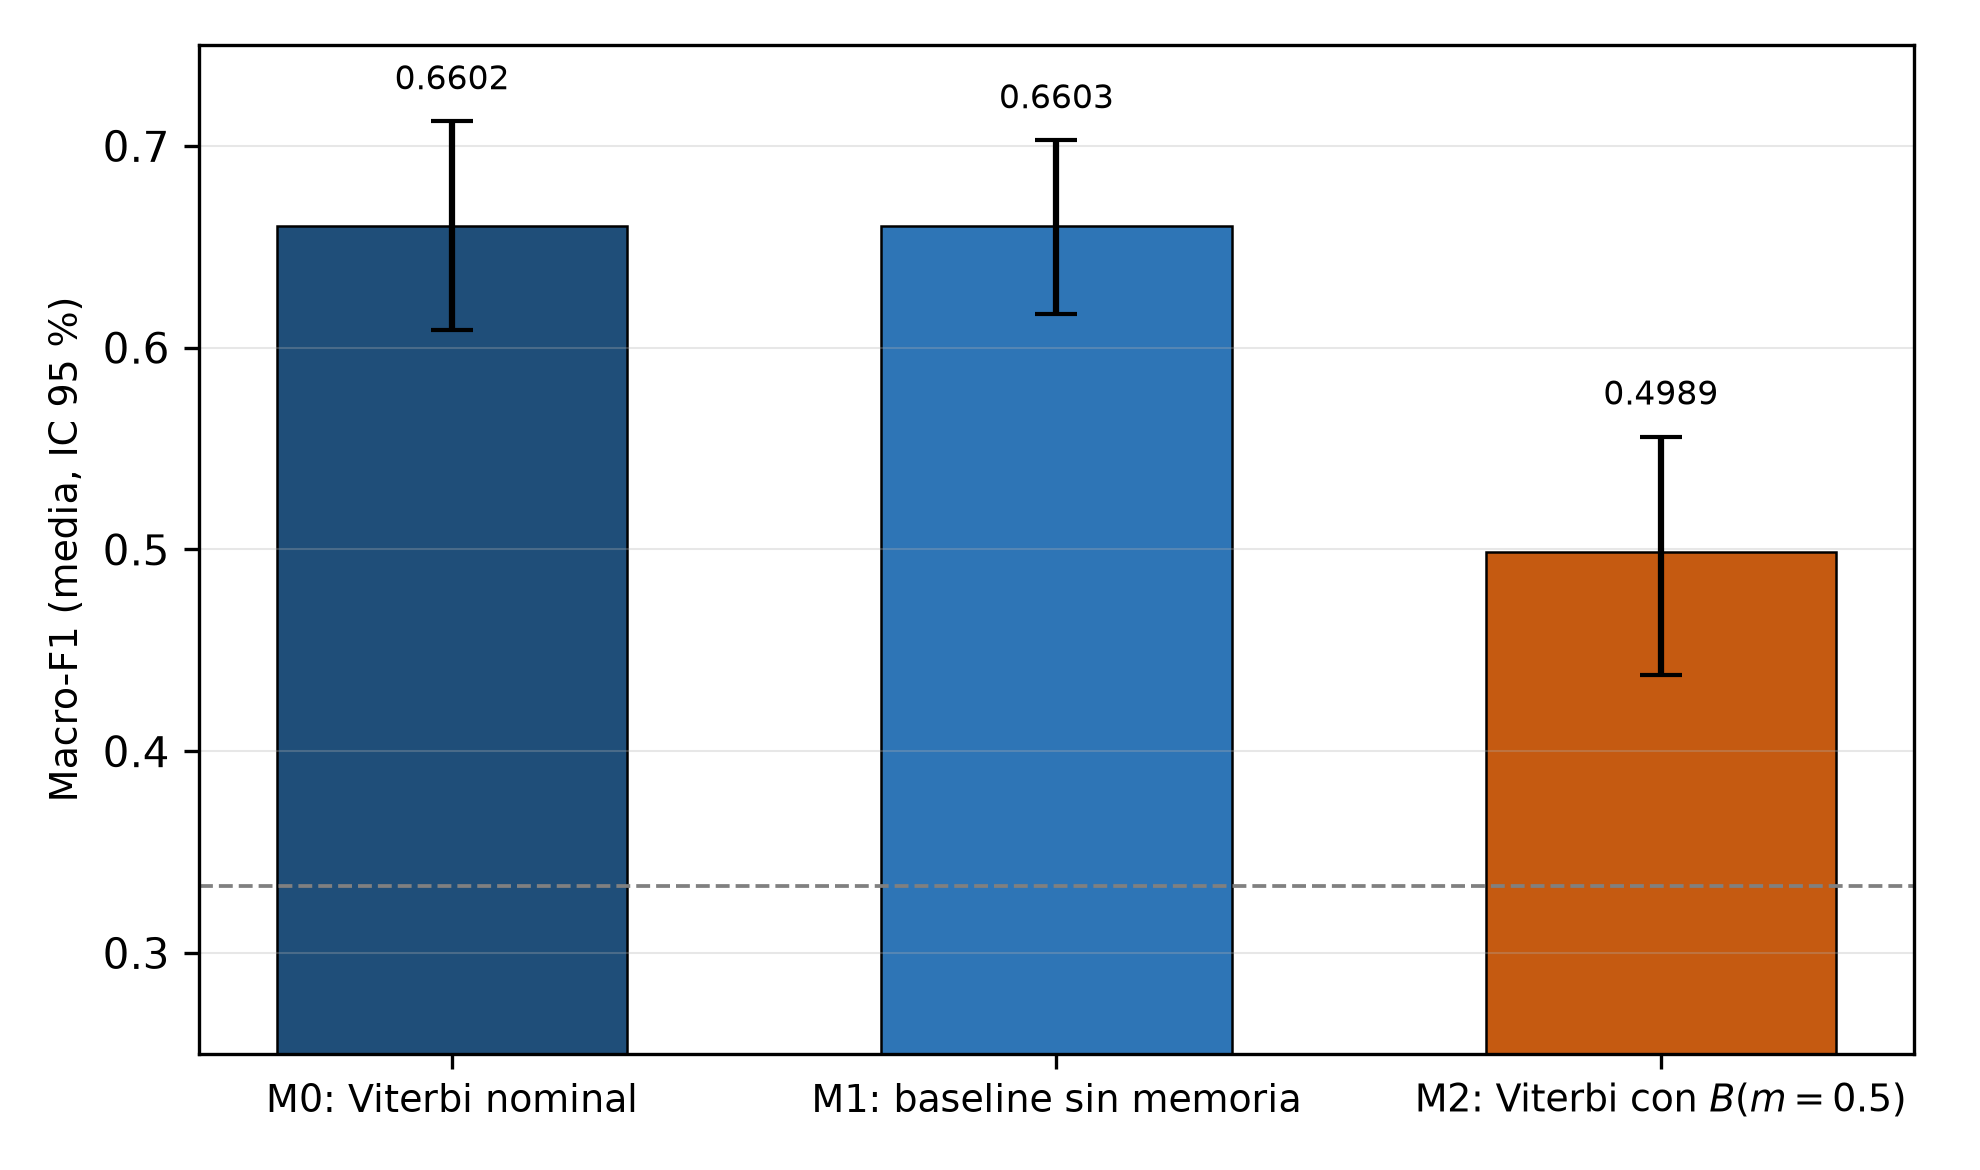
\includegraphics[width=0.78\textwidth]{outputs/fig_metricas_300dpi.png}
\caption{Macro-F1 por escenario (media e IC 95\,\%, 300 dpi). Datos simulados.}
\label{fig:metricas}
\end{figure}

\subsection{Contrastes pareados}

La Tabla~\ref{tab:contrastes} presenta los contrastes de Wilcoxon con corrección de Holm--Bonferroni y el delta de Cliff.

\begin{table}[H]
\centering
\caption{Contrastes pareados de macro-F1 (\(N=2000\) pares, \(\alpha=0.01\)).}
\label{tab:contrastes}
\small
\begin{tabular}{@{}lrrrrrr@{}}
\toprule
Contraste & \(\Delta\) media & \(W\) & \(p\) crudo & \(p\) Holm & \(\delta\) Cliff & Pos./Neg.\\
\midrule
M0 vs. M1 & \(-0.0002\) & 993\,219 & 0.7780 & 0.7780 & \(-0.0060\) & 994/1006\\
M0 vs. M2 & \(0.1612\) & 0 & \(<0.001\) & \(<0.001\) & \(1.0000\) & 2000/0\\
\bottomrule
\end{tabular}
\end{table}

El contraste M0--M1 no es significativo (\(p=0.7780\)) y su efecto es despreciable (\(|\delta|=0.0060\)). El contraste M0--M2 es significativo y máximo en la escala de Cliff (\(\delta=1.0\)): las 2000 secuencias favorecen a M0. El criterio C1 no se cumple; el criterio C2 sí.

\subsection{Matrices de confusión}

La Figura~\ref{fig:confusion} compara las matrices normalizadas por fila. M0 y M1 concentran la masa en la diagonal, con un patrón similar; M2 muestra mayor confusión entre Riesgo Moderado y las clases vecinas.

\begin{figure}[H]
\centering
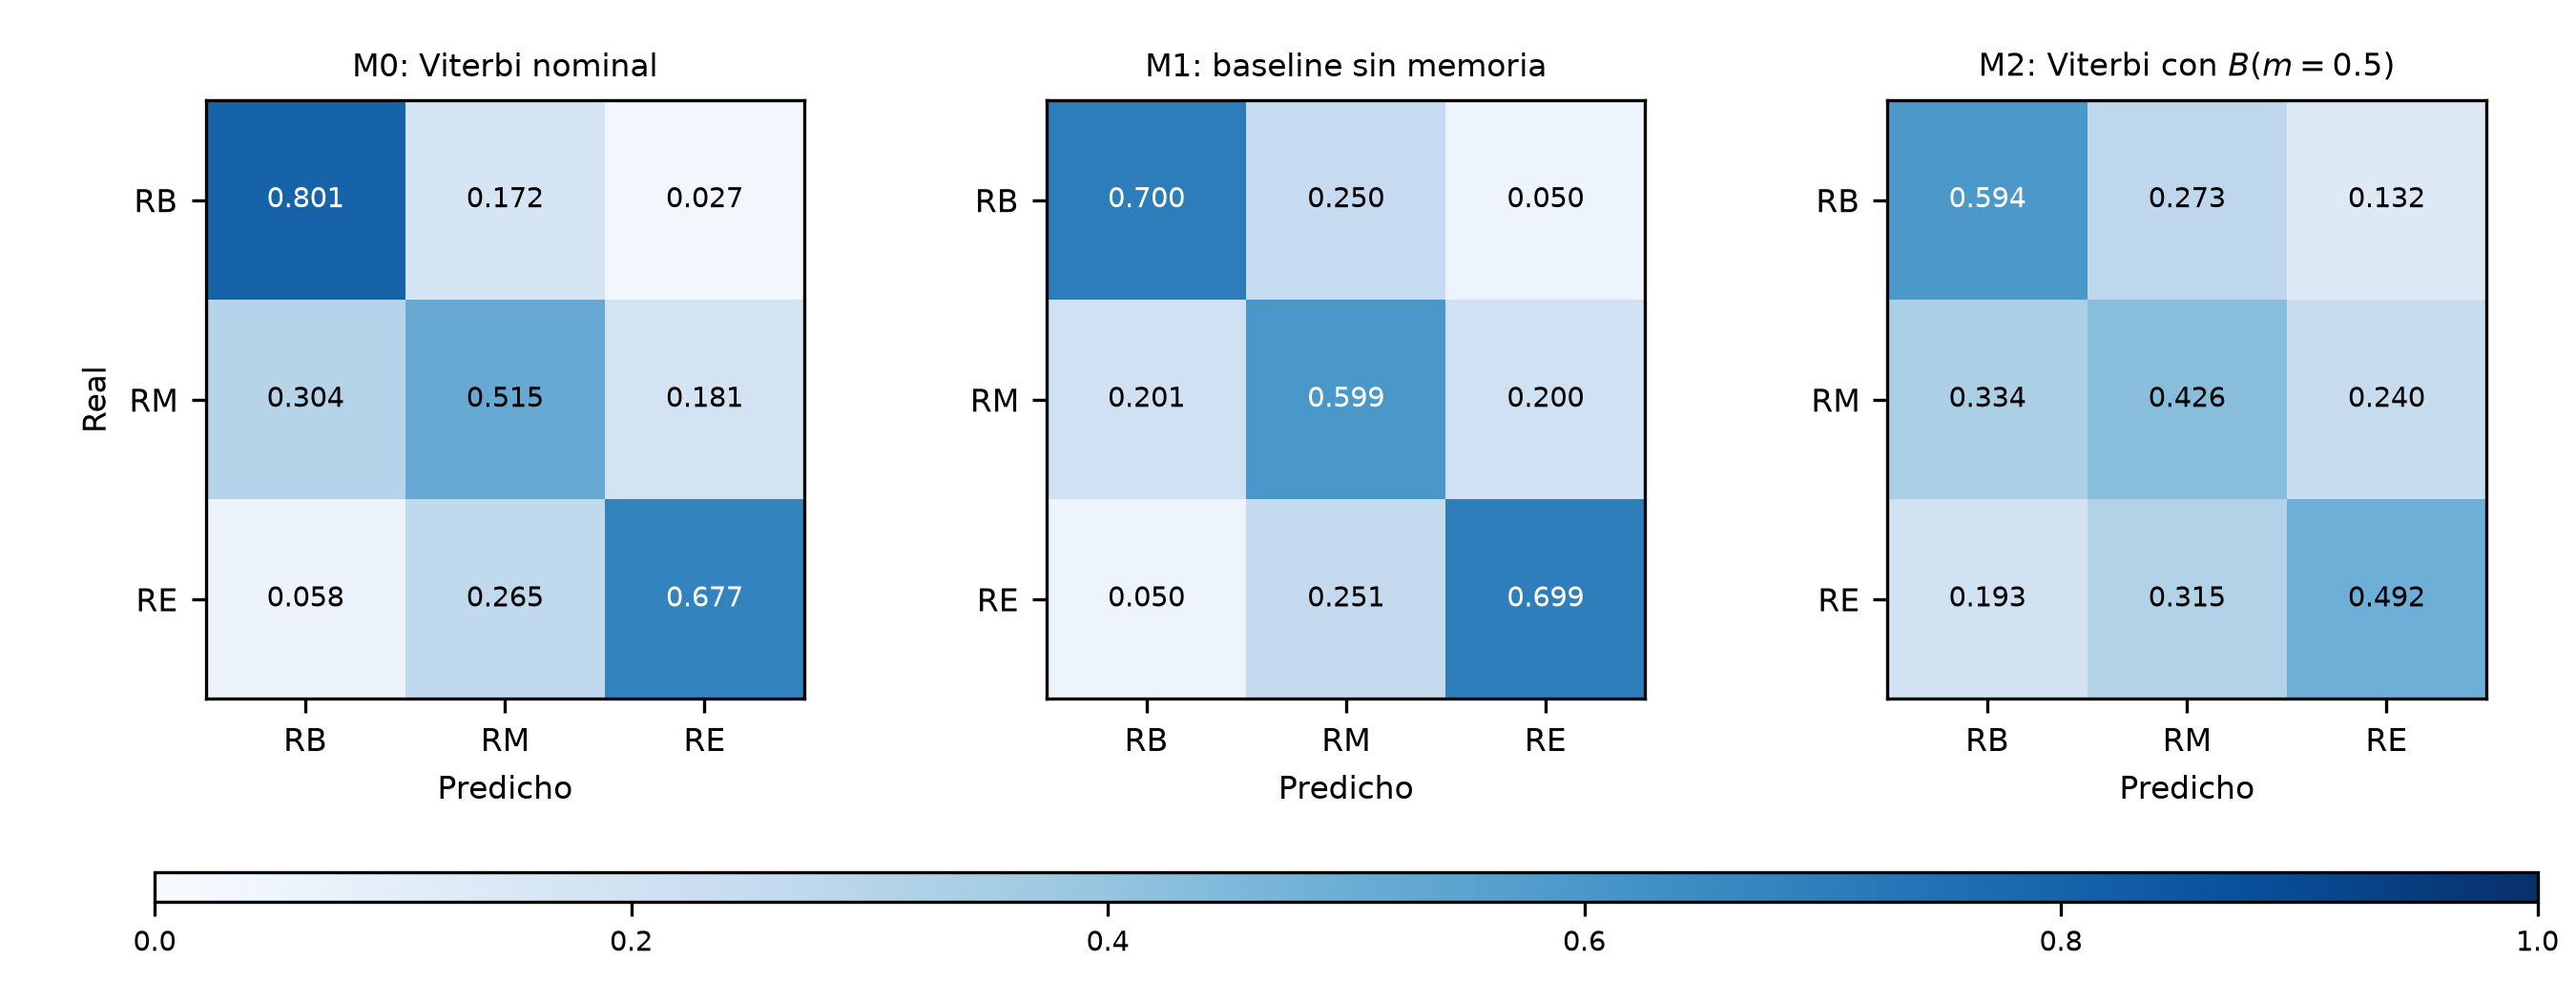
\includegraphics[width=\textwidth]{outputs/fig_confusion_300dpi.png}
\caption{Matrices de confusión normalizadas por fila para M0, M1 y M2 (300 dpi). Datos simulados.}
\label{fig:confusion}
\end{figure}

En M0, la diagonal es 0.8010, 0.5148 y 0.6766 para Riesgo Bajo, Moderado y Extremo. En M2, la diagonal baja a 0.5942, 0.4261 y 0.4923. La caída es coherente con la pérdida de separabilidad de \(B(0.5)\).

\subsection{Reproducibilidad}

La Tabla~\ref{tab:repro} resume los elementos que permiten regenerar los resultados. Los hashes SHA-256 se calcularon sobre los artefactos finales.

\begin{table}[H]
\centering
\caption{Evidencia de reproducibilidad y hashes SHA-256.}
\label{tab:repro}
\scriptsize
\begin{tabular}{@{}p{4.4cm}p{11.0cm}@{}}
\toprule
Elemento & Valor\\
\midrule
Semilla maestra & 42\\
Derivación & \texttt{np.random.SeedSequence(42).}\newline\texttt{spawn(2000)}\\
Mezcla de emisión & \(m=0.5\)\\
Nivel de significancia & \(\alpha=0.01\)\\
Corrección & Holm--Bonferroni\\
\texttt{experimento\_hmm\_resumen.json} & \texttt{2bad64f61c416aefdad53298f62e4de9}\newline\texttt{e93e8639918ef6b93558daec1860d289}\\
\texttt{tabla\_resumen\_manuscrito.csv} & \texttt{c5cee3deaf67d73cf25a03d79bfd7bbb}\newline\texttt{fec1d46a8d23f8c7dcdc525c841900f9}\\
\texttt{fig\_metricas\_300dpi.png} & \texttt{c66038cba94d677247131c7c8a0b5530}\newline\texttt{aa13c3074ecaa9ecbb693b833590ce54}\\
\texttt{fig\_confusion\_300dpi.png} & \texttt{bfd7329c55d118ea96b4b6fa348c5f07}\newline\texttt{83797a553faca4c5bf713e84f211b1a0}\\
\bottomrule
\end{tabular}
\end{table}

% ==================================================================
\section{Discusión}

\subsection{Por qué M0 y M1 son indistinguibles}

La equivalencia práctica entre Viterbi y la regla puntual tiene una explicación directa en la matriz de emisión. Cada fila de \(B\) tiene su máximo en la diagonal: 0.70 para Alta, 0.60 para Media y 0.70 para Baja, mientras que los valores fuera de la diagonal no superan 0.25. Por tanto, para cualquier observación \(o_t\), el estado que maximiza \(b_i(o_t)\) coincide con el estado asociado a esa humedad. El baseline M1 aplica exactamente ese argmax; M0 añade la transición \(A\), pero \(A\) también es diagonalmente dominante (0.70, 0.50 y 0.60) y la persistencia solo refuerza la misma asignación.

El resultado empírico es consistente con ese análisis: la diferencia media de macro-F1 es \(-0.000186\) (M1 ligeramente superior), \(p=0.7780\) y \(\delta=-0.0060\). En la práctica, la estructura de Markov no aporta una ventaja detectable en este régimen. Sí hay un intercambio en las métricas secundarias: M0 obtiene mayor exactitud (0.6728 frente a 0.6645), mientras que M1 obtiene mayor recall de Riesgo Extremo (0.6989 frente a 0.6738). La suavización temporal de Viterbi mejora la precisión global, pero absorbe algunos pasos extremos en estados vecinos.

\subsection{Por qué M2 cae con \(m=0.5\)}

La mezcla reduce la separación de las emisiones. En \(B(0.5)\), la diagonal toma valores 0.5167, 0.4667 y 0.5167, y los valores fuera de la diagonal quedan entre 0.1917 y 0.2917. Aunque la diagonal sigue siendo máxima, el margen entre la mejor y la segunda probabilidad se reduce de forma notable. Además, el decodificador M2 sigue usando \(B\) nominal, de modo que el modelo está mal especificado respecto al proceso que generó las observaciones: la ruta se elige con una verosimilitud que no corresponde a los datos.

La consecuencia cuantitativa es una caída de macro-F1 de 0.6602 a 0.4989, con diferencia media 0.1612, \(p<0.001\) y \(\delta=1.0\). Las 2000 secuencias favorecen a M0, sin empates. La exactitud de M2 (0.5123) y su recall de Riesgo Extremo (0.4908) confirman que la degradación no es un artefacto de una sola métrica. El hallazgo es coherente con la literatura: la calidad de las emisiones condiciona la decodificación, y la estructura temporal no compensa una matriz mal especificada.

\subsection{Contraste con la literatura}

Los trabajos aplicados revisados entrenan y evalúan con los mismos datos o reportan métricas heterogéneas \cite{wanjala2025,grammenos2025,tran2026,li2013,wang2026}. Nuestro diseño separa deliberadamente la decodificación de la estimación: no hay Baum--Welch y los tres escenarios reciben parámetros fijos. En ese sentido, el resultado no contradice a esos estudios; delimita una condición en la que la ventaja del HMM no se manifiesta. Los trabajos metodológicos \cite{nicosia2026,pouzo2025} advierten sobre la incertidumbre y la robustez, y este experimento añade una demostración controlada de que la dominancia diagonal de \(B\) puede hacer que un baseline sin memoria iguale a Viterbi.

\subsection{Amenazas a la validez}

\begin{itemize}
  \item \textbf{Constructo:} los estados son etiquetas puras y la humedad es ordinal; no hay una definición física de riesgo ni umbrales calibrados con datos de campo.
  \item \textbf{Interna:} los parámetros son hipotéticos y fijos; se evalúa un solo valor de mezcla (\(m=0.5\)) y una sola matriz \(A\). No se explora la sensibilidad a otras topologías.
  \item \textbf{Externa:} los datos son simulados; no se afirma validez ecológica ni capacidad de predicción de incendios reales.
  \item \textbf{Estadística:} las secuencias se generan por separado, pero las métricas por secuencia no capturan dependencias espaciales ni temporales de un territorio real.
  \item \textbf{De conclusión:} el estudio compara reglas de decodificación, no modelos entrenados; sus conclusiones no se extrapolan a sistemas operativos de alerta.
\end{itemize}

% ==================================================================
\section{Conclusiones y trabajo futuro}

\subsection{Respuesta a P1}

El riesgo dinámico puede representarse con \(\lambda=(S,V,A,B,\pi)\), donde \(S\) contiene las etiquetas Riesgo Bajo, Moderado y Extremo; \(V\) contiene Alta, Media y Baja; \(A\) describe la persistencia entre estados; \(B\) la relación entre estado y humedad; y \(\pi\) el prior inicial. La clave es que \(O_t\in V\): las observaciones son niveles de humedad, no estados latentes. Esta formalización permite calcular la verosimilitud con Forward, la ruta más probable con Viterbi y las posteriores marginales con Forward--Backward, sin inventar porcentajes ni umbrales físicos.

\subsection{Respuesta a P2}

Con parámetros fijos, M0 y M1 produjeron macro-F1 de 0.6602 y 0.6603, respectivamente; la diferencia media fue \(-0.000186\), con \(p=0.7780\) y \(\delta=-0.0060\). M2, con \(B(0.5)\), cayó a 0.4989. Los parámetros influyen de forma jerárquica en este caso: \(B\) determina la asignación porque su diagonal domina; \(A\) refuerza la persistencia, pero no cambia la decisión cuando la emisión es suficientemente informativa; y \(\pi\) pierde influencia a medida que \(T\) crece. La evidencia de que M1, que ignora \(A\) y \(\pi\), iguale a M0 respalda esa lectura.

\subsection{Respuesta a P3}

El protocolo es reproducible: semilla maestra 42, derivación \texttt{SeedSequence(42).spawn(2000)}, \(T=500\), \(N=2000\), \(m=0.5\), código y hashes SHA-256 documentados. Es sensible a la matriz de emisión: al pasar de \(B\) a \(B(0.5)\), la macro-F1 cae 0.1612, el contraste es significativo (\(p<0.001\)) y el delta de Cliff es 1.0. Frente al baseline sin memoria, el modelo no muestra superioridad bajo \(B\) nominal (\(p=0.7780\)); por tanto, la reproducibilidad no implica superioridad.

\subsection{Aportes y trabajo futuro}

El aporte principal es un protocolo auditable que separa estructura, emisiones y regla de decisión, junto con una comparación pareada y una tabla de verificación numérica. Como trabajo futuro se propone estimar \(A\), \(B\) y \(\pi\) con Baum--Welch sobre datos meteorológicos reales y partición por secuencia; explorar varios valores de \(m\) y distintas matrices \(A\); añadir análisis de sensibilidad a \(\pi\); incorporar validación externa con series de humedad de campo; y comparar Viterbi con la posterior marginal y con baselines supervisados. Cualquier extensión con datos reales requerirá una definición física del riesgo y una discusión explícita de las limitaciones de validez.

% ==================================================================
\begin{thebibliography}{10}

\bibitem{rabiner1989}
L. R. Rabiner, ``A tutorial on hidden Markov models and selected applications in speech recognition,'' \emph{Proceedings of the IEEE}, vol. 77, no. 2, pp. 257--286, Feb. 1989.

\bibitem{baum1970}
L. E. Baum, T. Petrie, G. Soules, and N. Weiss, ``A maximization technique occurring in the statistical analysis of probabilistic functions of Markov chains,'' \emph{The Annals of Mathematical Statistics}, vol. 41, no. 1, pp. 164--171, 1970.

\bibitem{wanjala2025}
D. W. Wanjala, J. W. Makokha, and G. W. Khamala, ``Anomaly detection in selected aerosol optical properties and associated climate variables using a multivariate hidden Markov model: A case study over Kenya,'' \emph{Open Access Library Journal}, vol. 12, Art. no. e14160, 2025, doi: 10.4236/oalib.1114160.

\bibitem{grammenos2025}
K. Grammenos, ``Hidden Markov models and their application in modeling rainfall occurrence,'' M.Sc. thesis, Athens University of Economics and Business, Athens, Greece, 2025, doi: 10.26219/heal.aueb.9331.

\bibitem{nicosia2026}
A. Nicosia, ``Tropical Viterbi tubes for decoding uncertainty in hidden Markov models,'' arXiv:2606.17181v1, 2026.

\bibitem{pouzo2025}
D. Pouzo, Z. Psaradakis, and M. Sola, ``On the robustness of mixture models in the presence of hidden Markov regimes with covariate-dependent transition probabilities,'' \emph{Econometric Theory}, vol. 41, pp. 1229--1243, 2025, doi: 10.1017/S0266466625100017.

\bibitem{tran2026}
H. T. Tran, G. T. Tran, H. T. Tran, N. M. Nguyen, and T. M. Phan, ``Integrating hidden Markov models and attention-based LSTM framework for regulation compliance in coastal water quality assessment: A case study in Vietnam,'' Preprints.org, 202605.1728.v1, 2026, doi: 10.20944/preprints202605.1728.v1.

\bibitem{li2013}
X. Li, J. Qian, and G. Wang, ``Fault prognostic based on hybrid method of state judgment and regression,'' \emph{Advances in Mechanical Engineering}, vol. 2013, Art. no. 149562, 2013.

\bibitem{deb2026}
B. Deb, S. Pandey, and P. Pakray, ``Quantum hidden Markov model for sequential analysis,'' \emph{Evolutionary Intelligence}, vol. 19, Art. no. 90, 2026, doi: 10.1007/s12065-026-01205-3.

\bibitem{wang2026}
J. Wang, Y. Wang, H. Wu, J. Gao, S. Xu, and D. Zou, ``StageGuard: Physiologically constrained sleep staging,'' in \emph{Proc. 32nd ACM SIGKDD Conf. Knowledge Discovery and Data Mining (KDD '26)}, vol. 2, pp. 12267--12278, 2026.

\end{thebibliography}

% ==================================================================
\appendix
\section{Tabla de verificación numérica}

La Tabla~\ref{tab:auditoria} contrasta las cifras reportadas en el cuerpo del manuscrito con los artefactos de \texttt{outputs/}. Todas las comprobaciones se realizaron sobre \texttt{experimento\_hmm\_resumen.json} y las figuras regeneradas con \texttt{scripts/build\_paper\_assets.py}.

\begin{longtable}{@{}>{\raggedright\arraybackslash}p{5.0cm}>{\raggedright\arraybackslash}p{2.6cm}>{\raggedright\arraybackslash}p{5.6cm}>{\raggedright\arraybackslash}p{1.9cm}@{}}
\caption{Verificación de cifras del manuscrito contra \texttt{outputs/}.}\label{tab:auditoria}\\
\toprule
Afirmación & Valor en texto & Fuente y campo & Estado\\
\midrule
\endfirsthead
\toprule
Afirmación & Valor en texto & Fuente y campo & Estado\\
\midrule
\endhead
\(T\) & 500 & \texttt{metadata.T} & Coincide\\
\(N\) & 2000 & \texttt{metadata.N} & Coincide\\
Semilla maestra & 42 & \texttt{metadata.master\_seed} & Coincide\\
Mezcla \(m\) & 0.5 & \texttt{metadata.mixing} & Coincide\\
M0 macro-F1 media & 0.6602 & \texttt{models.M0.macro\_f1.mean} & Coincide\\
M0 macro-F1 DE & 0.0263 & \texttt{models.M0.macro\_f1.sd} & Coincide\\
M0 macro-F1 mínimo & 0.5581 & \texttt{models.M0.macro\_f1.min} & Coincide\\
M0 macro-F1 máximo & 0.7356 & \texttt{models.M0.macro\_f1.max} & Coincide\\
M0 macro-F1 IC 95\,\% & [0.6089, 0.7121] & \texttt{ci\_low}, \texttt{ci\_high} & Coincide\\
M1 macro-F1 media & 0.6603 & \texttt{models.M1.macro\_f1.mean} & Coincide\\
M1 macro-F1 DE & 0.0216 & \texttt{models.M1.macro\_f1.sd} & Coincide\\
M1 macro-F1 IC 95\,\% & [0.6167, 0.7027] & \texttt{ci\_low}, \texttt{ci\_high} & Coincide\\
M2 macro-F1 media & 0.4989 & \texttt{models.M2.macro\_f1.mean} & Coincide\\
M2 macro-F1 DE & 0.0292 & \texttt{models.M2.macro\_f1.sd} & Coincide\\
M2 macro-F1 IC 95\,\% & [0.4380, 0.5558] & \texttt{ci\_low}, \texttt{ci\_high} & Coincide\\
M0 exactitud media & 0.6728 & \texttt{models.M0.accuracy.mean} & Coincide\\
M1 exactitud media & 0.6645 & \texttt{models.M1.accuracy.mean} & Coincide\\
M2 exactitud media & 0.5123 & \texttt{models.M2.accuracy.mean} & Coincide\\
M0 recall \(s_3\) & 0.6738 & \texttt{models.M0.recall\_s3.mean} & Coincide\\
M1 recall \(s_3\) & 0.6989 & \texttt{models.M1.recall\_s3.mean} & Coincide\\
M2 recall \(s_3\) & 0.4908 & \texttt{models.M2.recall\_s3.mean} & Coincide\\
M0\(-\)M1 diferencia & \(-0.000186\) & \texttt{comparisons.M0\_vs\_M1} & Coincide\\
M0\(-\)M1 \(p\) & 0.7780 & \texttt{comparisons.M0\_vs\_M1} & Coincide\\
M0\(-\)M1 \(\delta\) Cliff & \(-0.0060\) & \texttt{comparisons.M0\_vs\_M1} & Coincide\\
M0\(-\)M2 diferencia & 0.1612 & \texttt{comparisons.M0\_vs\_M2} & Coincide\\
M0\(-\)M2 \(p\) & \(<0.001\) & \texttt{comparisons.M0\_vs\_M2} & Coincide\\
M0\(-\)M2 \(\delta\) Cliff & 1.0000 & \texttt{comparisons.M0\_vs\_M2} & Coincide\\
M0 diagonal confusión & 0.8010 / 0.5148 / 0.6766 & \texttt{models.M0} & Coincide\\
M2 diagonal confusión & 0.5942 / 0.4261 / 0.4923 & \texttt{models.M2} & Coincide\\
Criterio C1 & No cumple & \texttt{criteria.criterion\_1} & Coincide\\
Criterio C2 & Cumple & \texttt{criteria.criterion\_2} & Coincide\\
\bottomrule
\end{longtable}

\noindent La auditoría automatizada de las 66 cifras se reproduce con \texttt{audit\_manuscript.py}.\par
\noindent El detalle está en \texttt{auditoria\_final.md}.\par
\noindent\textbf{Conteo del resumen:} 228 palabras (rango 150--250).\par
\noindent\textbf{Extensión:} 14 páginas de cuerpo, sin Referencias ni Anexo (rango 10--15).

% ==================================================================
\clearpage
\section{Guion del video pitch}

El video pitch tiene una duración objetivo de 2:30 minutos, en formato MP4 1920$\times$1080 (16:9 horizontal, H.264 + AAC) y un ritmo de lectura cercano a 130 palabras por minuto. Se reparte en partes iguales entre los tres integrantes. Todas las cifras citadas provienen de \texttt{outputs/experimento\_hmm\_resumen.json} y coinciden con las auditadas en el Anexo~A. El guion completo, con las indicaciones visuales detalladas, se conserva en \texttt{docs/guion\_pitch.md}.

\begin{table}[H]
\centering
\caption{Reparto y tiempos del video pitch.}
\label{tab:pitch}
\small
\begin{tabular}{@{}p{4.6cm}p{1.1cm}p{3.4cm}p{1.9cm}p{1.3cm}@{}}
\toprule
Integrante & Bloque & Tema & Ventana & Duración\\
\midrule
Oscar A. De la Pava Suarez & 1 & Gancho & 0:00--0:13 & 13 s\\
Oscar A. De la Pava Suarez & 2 & Motivación e impacto & 0:13--0:32 & 19 s\\
Oscar A. De la Pava Suarez & 3 & Solución propuesta & 0:32--0:51 & 19 s\\
Anderson J. Ospina Cardona & 4 & Metodología y diseño & 0:51--1:15 & 24 s\\
Anderson J. Ospina Cardona & 5 & Resultado clave & 1:15--1:42 & 27 s\\
Kevin A. Valencia Daza & 6 & Aporte científico & 1:42--2:08 & 26 s\\
Kevin A. Valencia Daza & 7 & Cierre & 2:08--2:30 & 22 s\\
\bottomrule
\end{tabular}
\end{table}

\subsection*{Integrante 1 --- Contexto y modelo (0:00--0:51)}

\textbf{Bloque 1. Gancho (0:00--0:13).}
\begin{quote}\small
Imaginen un bosque donde solo podemos medir la humedad: alta, media o baja. El riesgo real ---bajo, moderado o extremo--- permanece oculto. ¿Podemos inferirlo con matemáticas?
\end{quote}
\noindent\emph{[Cámara del presentador, plano medio. Fondo de bosque con iconos de humedad. Rótulo: ``Riesgo oculto $\rightarrow$ ¿inferible?''.]}

\medskip
\textbf{Bloque 2. Motivación e impacto (0:13--0:32).}
\begin{quote}\small
Antes de llevar un modelo así a una alerta real, necesitamos saber cuánto depende de sus supuestos. Un modelo que parece acertado puede fallar en silencio si sus observaciones pierden calidad. Medir esa sensibilidad es tan importante como medir el acierto.
\end{quote}
\noindent\emph{[Screencast de \texttt{fig\_metricas\_300dpi.png} con zoom al eje macro-F1; corte a cámara. Rótulo: ``Sensibilidad antes que despliegue''.]}

\medskip
\textbf{Bloque 3. Solución propuesta (0:32--0:51).}
\begin{quote}\small
Proponemos un HMM discreto: lambda igual a $S$, $V$, $A$, $B$ y $\pi$. Tres estados ocultos de riesgo, tres observaciones ordinales de humedad, matriz de transición $A$, matriz de emisión $B$ y prior $\pi$. Decodificamos con Viterbi en espacio logarítmico para evitar desbordamientos numéricos.
\end{quote}
\noindent\emph{[Diagrama animado del HMM: estados RB--RM--RE, transiciones $A$, emisiones $B$ hacia Alta--Media--Baja y vector $\pi$. Cierre con el Algoritmo~1 resaltando el uso de logaritmos.]}

\subsection*{Integrante 2 --- Experimento y resultados (0:51--1:42)}

\textbf{Bloque 4. Metodología y diseño experimental (0:51--1:15).}
\begin{quote}\small
En una frase: simulamos un HMM con parámetros fijos y comparamos tres reglas pareadas. Generamos dos mil secuencias, cada una de quinientos pasos: M0 decodifica con Viterbi nominal, M1 clasifica cada paso solo con $B$, sin memoria, y M2 usa Viterbi sobre observaciones degradadas con $m$ igual a cero punto cinco.
\end{quote}
\noindent\emph{[Cámara y screencast de \texttt{src/simulation.py} con \texttt{DEFAULT\_T}, \texttt{DEFAULT\_N} y \texttt{ALTERED\_MIXING}. Inserto del diagrama de flujo F1--F7 (Figura~1). Rótulo: ``$T=500$, $N=2000$, pareado''.]}

\medskip
\textbf{Bloque 5. Resultado clave (1:15--1:42).}
\begin{quote}\small
Bajo $B$ nominal, M0 y M1 son estadísticamente indistinguibles: macro-F1 de 0.6602 frente a 0.6603, con $p$ igual a 0.778 y delta de Cliff de menos 0.006. En cambio, M2 cae a 0.4989: una diferencia de 0.1612, $p$ menor que 0.001 y delta de Cliff de 1.0. Las dos mil secuencias favorecen a M0. No hay empates.
\end{quote}
\noindent\emph{[Gráfica de barras a 300 dpi (\texttt{fig\_metricas\_300dpi.png}) con las tres medias y sus IC. Luego la Tabla~4, resaltando la fila M0 vs.\ M2. Señalizar en pantalla: ``Datos simulados --- outputs/''.]}

\subsection*{Integrante 3 --- Aporte y cierre (1:42--2:30)}

\textbf{Bloque 6. Aporte científico (1:42--2:08).}
\begin{quote}\small
El aporte no es que el HMM gane, sino demostrar cuándo no gana. Con Wilcoxon pareado, Holm--Bonferroni y delta de Cliff separamos señal de azar. Y todo es reproducible: código, semillas, hashes SHA-256 y auditoría de las sesenta y seis cifras. Cualquiera puede repetir el experimento y obtener los mismos números.
\end{quote}
\noindent\emph{[Screencast de la auditoría final recorriendo la tabla de verificación; corte al manifiesto con los hashes. Rótulo: ``66 cifras auditadas, 15 pruebas''.]}

\medskip
\textbf{Bloque 7. Cierre (2:08--2:30).}
\begin{quote}\small
Respondiendo: el riesgo se representa con un HMM discreto; los parámetros influyen de forma jerárquica, con $B$ dominando; y el modelo es reproducible pero sensible a la calidad de las emisiones. El alcance es simulado: no afirmamos predicción de incendios reales. El siguiente paso es estimar $A$, $B$ y $\pi$ con Baum--Welch sobre datos meteorológicos reales. Gracias.
\end{quote}
\noindent\emph{[Cámara del presentador a plano medio, cierre con tarjeta final: título, los tres nombres, correos institucionales y URL del repositorio. Fundido a negro.]}

\end{document}
